% =============================================================================
% Supervised Learning Presentation using Sustainability Lab Beamer Class
% =============================================================================

\documentclass{sustainabilitylab}

% =============================================================================
% PRESENTATION METADATA
% =============================================================================

\title{Supervised Learning for Environmental Applications}
\subtitle{From Theory to Practice in Sustainability Research}
\author{Nipun Batra}
\institute{Sustainability Lab \\ IIT Gandhinagar}
\date{July 2025}

% =============================================================================
% DOCUMENT CONTENT
% =============================================================================

\begin{document}

% Title slide
\begin{frame}
  \titlepage
\end{frame}

% Table of contents
\begin{frame}{Outline}
  \tableofcontents
\end{frame}

% =============================================================================
% SECTION 1: INTRODUCTION
% =============================================================================

\section{Introduction to Supervised Learning}

\begin{frame}{What is Supervised Learning?}

Supervised learning uses labeled training data to predict outcomes on new data.

\begin{itemize}
  \item \textbf{Classification}: Predicting discrete categories
  \item \textbf{Regression}: Predicting continuous values
  \item \textbf{Key Components}: Features, labels, model, loss function
\end{itemize}

\end{frame}

\begin{frame}{Environmental Applications}

\begin{itemize}
  \item Energy consumption prediction
  \item Air quality classification
  \item Species identification from sensor data
  \item Climate pattern recognition
\end{itemize}

\end{frame}

\begin{frame}{Supervised Learning Workflow}

\begin{center}
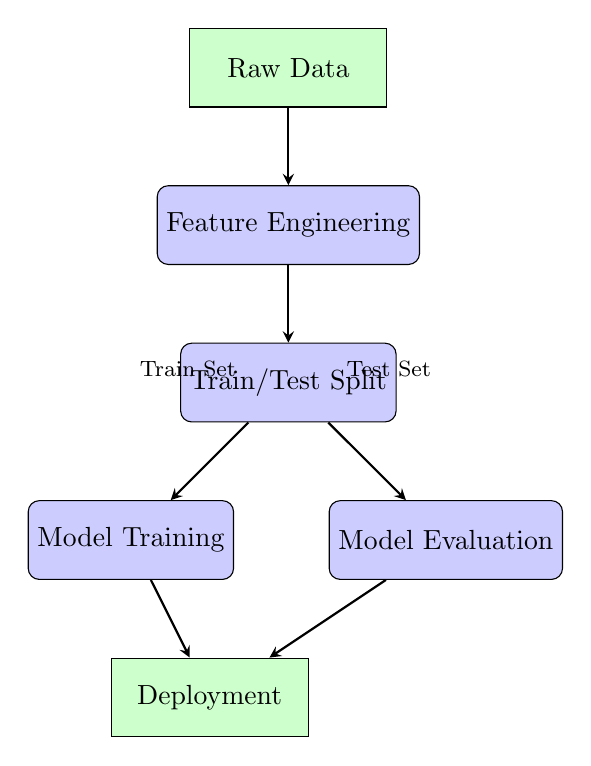
\begin{tikzpicture}[node distance=2cm, scale=0.85]
  % Define styles
  \tikzstyle{process} = [rectangle, rounded corners, minimum width=2.5cm, minimum height=1cm, 
                         text centered, draw=black, fill=blue!20]
  \tikzstyle{data} = [rectangle, minimum width=2.5cm, minimum height=1cm, 
                      text centered, draw=black, fill=green!20]
  \tikzstyle{arrow} = [thick,->,>=stealth]
  
  % Nodes
  \node (data) [data] {Raw Data};
  \node (features) [process, below of=data] {Feature Engineering};
  \node (split) [process, below of=features] {Train/Test Split};
  \node (train) [process, below of=split, xshift=-2cm] {Model Training};
  \node (eval) [process, below of=split, xshift=2cm] {Model Evaluation};
  \node (deploy) [data, below of=train, xshift=1cm] {Deployment};
  
  % Arrows
  \draw [arrow] (data) -- (features);
  \draw [arrow] (features) -- (split);
  \draw [arrow] (split) -- (train);
  \draw [arrow] (split) -- (eval);
  \draw [arrow] (train) -- (deploy);
  \draw [arrow] (eval) -- (deploy);
  
  % Labels on arrows
  \node at (-1.5,-4.5) {\footnotesize Train Set};
  \node at (1.5,-4.5) {\footnotesize Test Set};
\end{tikzpicture}
\end{center}

\textbf{Key Steps:} Data preparation, model selection, validation, deployment

\end{frame}

% =============================================================================
% SECTION 2: ALGORITHMS
% =============================================================================

\section{Core Algorithms}

\begin{frame}{Linear Regression}

\textbf{Mathematical Form:}
$$y = \beta_0 + \beta_1 x_1 + \beta_2 x_2 + \ldots + \beta_n x_n + \epsilon$$

\textbf{Key Properties:}
\begin{itemize}
  \item Simple and interpretable
  \item Fast training and prediction
  \item Assumes linear relationships
  \item Good baseline model
\end{itemize}

\end{frame}

\begin{frame}{Energy Consumption Example}

\textbf{Variables:}
\begin{itemize}
  \item $y$: Daily energy usage (kWh)
  \item $x_1$: Temperature (°C)
  \item $x_2$: Humidity (\%)
  \item $x_3$: Number of occupants
\end{itemize}

\vspace{1cm}
\textit{Model learns how each factor influences energy consumption}

\end{frame}

\begin{frame}[fragile]{Implementation Example}

\begin{codebox}
from sklearn.linear_model import LinearRegression
from sklearn.model_selection import train_test_split
import pandas as pd
from sklearn.metrics import mean_squared_error, r2_score

# Load data
data = pd.read_csv('energy_consumption.csv')
X = data[['temperature', 'humidity', 'occupancy']]
y = data['energy_kwh']

# Split and train
X_train, X_test, y_train, y_test = train_test_split(
    X, y, test_size=0.2, random_state=42)

model = LinearRegression()
model.fit(X_train, y_train)

# Evaluate
y_pred = model.predict(X_test)
mse = mean_squared_error(y_test, y_pred)
r2 = r2_score(y_test, y_pred)
\end{codebox}
\end{frame}

\begin{frame}{Decision Trees}

\textbf{How it works:}
\begin{itemize}
  \item Splits data based on feature values
  \item Creates if-then rules automatically
  \item Handles non-linear relationships
  \item Easy to interpret and visualize
\end{itemize}

\textbf{Advantages:}
\begin{itemize}
  \item No assumptions about data distribution
  \item Handles mixed data types
  \item Built-in feature selection
\end{itemize}

\end{frame}

\begin{frame}{Decision Tree Example}

\texttt{
\footnotesize
if PM2.5 > 35:\\
\quad if NO2 > 40:\\
\quad \quad class = "Poor"\\
\quad else:\\
\quad \quad class = "Moderate"\\
else:\\
\quad if O3 < 80:\\
\quad \quad class = "Good"\\
\quad else:\\
\quad \quad class = "Moderate"
}

\end{frame}

\begin{frame}{Neural Networks}

\textbf{Architecture:}
\begin{itemize}
  \item Interconnected layers of neurons
  \item Non-linear activation functions
  \item Learns complex patterns automatically
  \item Requires more data but higher accuracy
\end{itemize}

\begin{center}
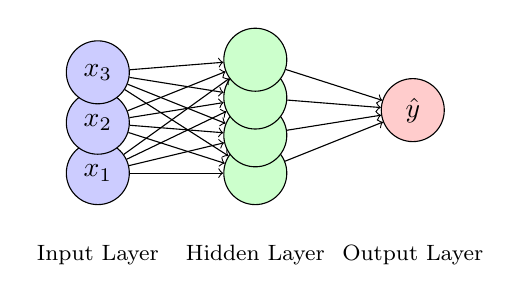
\begin{tikzpicture}[scale=0.8]
  % Define layer positions
  \def\layersep{2.5cm}
  
  % Input layer
  \foreach \y in {1,2,3}
    \node[circle,draw,minimum size=8mm,fill=blue!20] (I-\y) at (0,\y*0.8) {$x_\y$};
  
  % Hidden layer
  \foreach \y in {1,2,3,4}
    \node[circle,draw,minimum size=8mm,fill=green!20] (H-\y) at (\layersep,\y*0.6+0.2) {};
  
  % Output layer
  \node[circle,draw,minimum size=8mm,fill=red!20] (O) at (2*\layersep,1.8) {$\hat{y}$};
  
  % Connect input to hidden
  \foreach \source in {1,2,3}
    \foreach \dest in {1,2,3,4}
      \draw[->] (I-\source) -- (H-\dest);
  
  % Connect hidden to output
  \foreach \source in {1,2,3,4}
    \draw[->] (H-\source) -- (O);
  
  % Labels
  \node at (0,-0.5) {\footnotesize Input Layer};
  \node at (\layersep,-0.5) {\footnotesize Hidden Layer};
  \node at (2*\layersep,-0.5) {\footnotesize Output Layer};
\end{tikzpicture}
\end{center}

\end{frame}

\begin{frame}{Neural Network Applications}

\textbf{Environmental Use Cases:}
\begin{itemize}
  \item \textbf{Air Quality Prediction}: Multi-pollutant forecasting
  \item \textbf{Energy Load Forecasting}: Grid demand prediction
  \item \textbf{Climate Modeling}: Temperature and precipitation patterns
  \item \textbf{Species Classification}: Biodiversity monitoring from audio/images
\end{itemize}

\vspace{0.5cm}

\textbf{Architecture Considerations:}
\begin{itemize}
  \item \textbf{Feedforward}: Standard prediction tasks
  \item \textbf{LSTM/RNN}: Time series data (weather, energy)
  \item \textbf{CNN}: Satellite imagery analysis
  \item \textbf{Transformer}: Multi-modal environmental data
\end{itemize}

\end{frame}

% =============================================================================
% SECTION 3: EVALUATION
% =============================================================================

\section{Model Evaluation}

\begin{frame}{Performance Metrics}

\begin{table}[h]
\centering
\begin{tabular}{lcc}
\toprule
\textbf{Metric} & \textbf{Regression} & \textbf{Classification} \\
\midrule
Primary & Mean Squared Error & Accuracy \\
Secondary & R² Score & F1-Score \\
Interpretable & Mean Absolute Error & Confusion Matrix \\
\bottomrule
\end{tabular}
\end{table}

\textbf{Key Considerations:}
\begin{itemize}
  \item Choose metrics relevant to your problem
  \item Consider class imbalance in classification
  \item Use cross-validation for robust estimates
\end{itemize}

\end{frame}

\begin{frame}{Cross-Validation Results}
\frametitle{Model Comparison}

\begin{table}[h]
\centering
\begin{tabular}{lccc}
\toprule
\textbf{Algorithm} & \textbf{Energy Prediction} & \textbf{Air Quality} & \textbf{Training Time} \\
& \textbf{(R² Score)} & \textbf{(Accuracy)} & \textbf{(seconds)} \\
\midrule
Linear Regression & 0.73 & -- & 0.02 \\
Logistic Regression & -- & 0.84 & 0.05 \\
Decision Tree & 0.68 & 0.79 & 0.12 \\
Random Forest & 0.81 & 0.87 & 2.45 \\
Support Vector Machine & 0.76 & 0.85 & 12.30 \\
Neural Network & 0.83 & 0.89 & 45.60 \\
\bottomrule
\end{tabular}
\caption{5-fold cross-validation results on sustainability datasets}
\end{table}

\textbf{Key Insights:}
\begin{itemize}
  \item Random Forest offers good balance of accuracy and speed
  \item Neural networks achieve highest accuracy but require more computation
  \item Linear models remain competitive for simpler problems
\end{itemize}

\end{frame}

% =============================================================================
% SECTION 4: APPLICATIONS
% =============================================================================

\section{Real-World Applications}

\begin{frame}{Smart Grid Optimization}

\textbf{Problem Setup:}
\begin{itemize}
  \item Predict hourly electricity demand
  \item Features: weather, time, historical usage
  \item Goal: Optimize energy generation and storage
\end{itemize}

\textbf{Data Sources:}
\begin{itemize}
  \item Smart meter readings (10M+ households)
  \item Weather station data
  \item Calendar information
  \item Economic indicators
\end{itemize}

\end{frame}

\begin{frame}{Grid Optimization Results}

\textbf{Model Performance:}
\begin{itemize}
  \item Accuracy: 92\% within 5\% error
  \item Cost savings: \$2.3M annually
  \item CO2 reduction: 15,000 tons/year
\end{itemize}

\textbf{Deployment:}
\begin{itemize}
  \item Real-time predictions every 15 minutes
  \item Automatic model retraining weekly
  \item Integration with grid control systems
\end{itemize}

\end{frame}

\begin{frame}{Feature Importance Analysis}

\textbf{Feature Importance (Random Forest):}

\begin{tabular}{lr}
\toprule
\textbf{Feature} & \textbf{Importance} \\
\midrule
Hour of day & 0.34 \\
Temperature & 0.22 \\
Day of week & 0.18 \\
Previous day usage & 0.12 \\
Humidity & 0.08 \\
Wind speed & 0.04 \\
Holiday indicator & 0.02 \\
\bottomrule
\end{tabular}

\end{frame}

\begin{frame}{Key Insights}

\textbf{Analysis Results:}
\begin{itemize}
  \item Time patterns dominate (52\% combined)
  \item Weather matters, especially temperature
  \item Historical usage provides context
  \item Complex interactions between features
\end{itemize}

\textbf{Business Impact:}
\begin{itemize}
  \item Better demand forecasting
  \item Reduced energy waste
  \item Improved grid stability
\end{itemize}

\end{frame}

% =============================================================================
% SECTION 5: CHALLENGES
% =============================================================================

\section{Challenges \& Future Directions}

\begin{frame}{Current Challenges}

\textbf{Data Quality Issues:}
\begin{itemize}
  \item Missing sensor readings
  \item Measurement errors and drift
  \item Inconsistent data collection
  \item Privacy and access constraints
\end{itemize}

\textbf{Model Limitations:}
\begin{itemize}
  \item Assumption violations
  \item Overfitting to training data
  \item Poor generalization
\end{itemize}

\end{frame}

\begin{frame}{Environmental Complexity}

\textbf{Environmental Challenges:}
\begin{itemize}
  \item Non-stationary patterns (climate change)
  \item Multi-scale temporal effects
  \item Spatial dependencies
  \item Extreme events and outliers
\end{itemize}

\textbf{Practical Constraints:}
\begin{itemize}
  \item Computational resources
  \item Real-time requirements
  \item Model maintenance and updates
  \item Stakeholder acceptance
\end{itemize}

\end{frame}

\begin{frame}{Future Research Directions}

\textbf{Advanced Methodologies:}
\begin{itemize}
  \item \textbf{Transfer Learning}: Adapt models across regions
  \item \textbf{Federated Learning}: Distributed sensor networks
  \item \textbf{Physics-Informed ML}: Incorporate domain knowledge
  \item \textbf{Uncertainty Quantification}: Better risk assessment
\end{itemize}

\textbf{Integration Opportunities:}
\begin{itemize}
  \item Multi-modal data fusion
  \item Real-time learning and adaptation
  \item Human-in-the-loop decision making
  \item Explainable AI for policy makers
\end{itemize}

\end{frame}

\begin{frame}{Impact Areas}

\textbf{Sustainability Applications:}
\begin{itemize}
  \item Climate change mitigation and adaptation
  \item Sustainable urban planning
  \item Renewable energy optimization
  \item Biodiversity conservation
\end{itemize}

\end{frame}

% =============================================================================
% CONCLUSION
% =============================================================================

\section{Conclusion}

\begin{frame}{Key Takeaways}

\textbf{What We've Learned:}
\begin{itemize}
  \item Supervised learning provides powerful tools for environmental problems
  \item Model selection depends on data characteristics and requirements
  \item Evaluation must consider domain-specific metrics
  \item Real-world deployment requires practical considerations
\end{itemize}

\textbf{Best Practices:}
\begin{itemize}
  \item Start simple, then increase complexity
  \item Invest in data quality and understanding
  \item Use appropriate validation strategies
  \item Consider interpretability alongside accuracy
\end{itemize}

\end{frame}

\begin{frame}{Questions and Discussion}

\begin{center}
\Large
\textbf{How can we better leverage supervised learning for sustainability challenges?}
\end{center}

\end{frame}

\end{document}